To integrate the Multidomain Extension, begin by cloning the repository: \newline\newline
\texttt{git clone <LINK\_TO\_FINAL\_REPO>}

\subsubsection{Step 1: Create the C++ Class in Unreal Engine}
\begin{enumerate}
    \item Launch the \texttt{.uproject} file (e.g., \texttt{Blocks.uproject}) that utilizes the Cosys-AirSim plugin.
    \item Initialize the class: 
    \begin{itemize}
        \item Navigate to \texttt{Tools} $\rightarrow$ \texttt{New C++ Class...}
        \item Select \texttt{All Classes}, search for \textbf{\texttt{SimModeWorldBase}}, and click \texttt{Next}.
    \end{itemize}
    \item Configure the files:
    \begin{description}
        \item[Name:] \texttt{SimModeWorldMultidomain}
        \item[Path:] \texttt{.../Plugins/AirSim/Source/Vehicles/Multidomain/}
    \end{description}
    \begin{figure}[H]
    \centering
    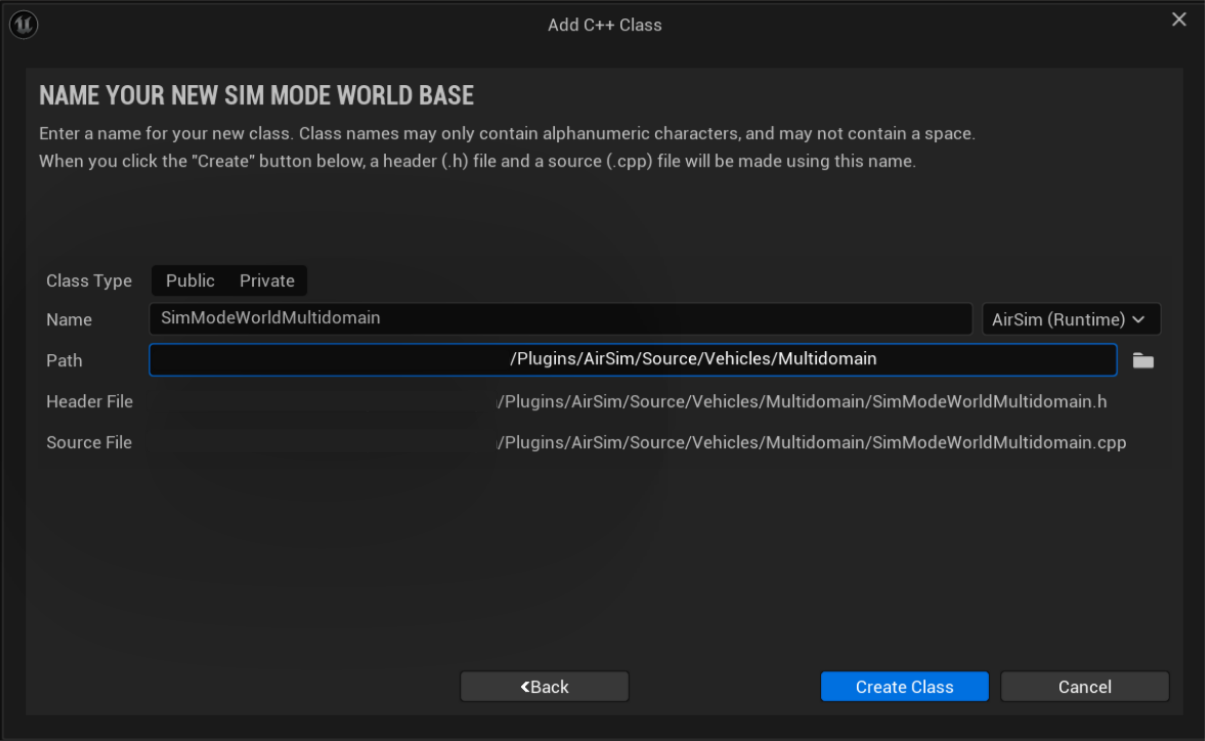
\includegraphics[width=0.7\textwidth]{graphics/new_class.png}
    \caption{\small Unreal Engine dialog showing the class name and destination path during extension integration.}
    \label{fig:ue_add_cpp_class_plugin}
    \end{figure}
    \item Click \texttt{Create Class} and wait for the \textit{Live Coding} notification to complete.
\end{enumerate}



\subsubsection{Step 2: File Replacement Registry}
\noindent
Replace the following existing files in your local directory with the modified versions from the cloned repository:

\begin{table}[H]
\centering
\small
\begin{tabular}{lll}
\toprule
\textbf{Directory Path (.../Plugins/AirSim/Source/)} & \textbf{Files to Replace} \\ \midrule
\texttt{AirLib/include/common/}        & \texttt{AirSimSettings.hpp} \\
\texttt{SimMode/}                      & \texttt{SimModeBase.*}, \texttt{SimModeWorldBase.*} \\
\texttt{SimHUD/}                       & \texttt{SimHUD.cpp} \\
\texttt{Vehicles/Car/}                 & \texttt{SimModeCar.*} \\
\texttt{Vehicles/Multidomain/}         & \texttt{SimModeWorldMultidomain.*} \\
\texttt{Vehicles/Multirotor/}          & \texttt{SimModeWorldMultirotor.*} \\
\texttt{Vehicles/ComputerVision/}      & \texttt{SimModeComputerVision.*} \\
\texttt{Vehicles/SkidVehicle/}         & \texttt{SimModeSkidVehicle.*} \\ \bottomrule
\end{tabular}
\end{table}

\subsubsection{Step 3: Clean and Rebuild Environment}
\begin{enumerate}[label=\alph*.]
     \item Navigate to \texttt{Plugins/AirSim/} and delete its specific \texttt{Binaries} and \texttt{Intermediate} folders.
    \item Delete the following folders from your project root: 
    \texttt{Binaries}, \texttt{Intermediate}, \texttt{Saved}, \texttt{DerivedDataCache}.
    \item Delete the existing \texttt{.sln} file from your project root.
    \item Right-click the \texttt{.uproject} file $\rightarrow$ \texttt{Show More Options} $\rightarrow$ \texttt{Generate Visual Studio project files}.
    \item Open the new \texttt{.sln}. Ensure the configuration is set to \textbf{\texttt{DevelopmentEditor}} on \textbf{\texttt{Win64}}. Press \texttt{F5} to build and launch the editor.
\end{enumerate}
